%\documentclass[manuscript]{aastex}
\documentclass[iop,useAMES,usenatbig]{emulateapj}

\shorttitle{Simultaneous multi-band transits of WD1145+017}
\shortauthors{Zhou et al.}


%%% packages
\usepackage{graphicx}
\usepackage{amsmath}
\usepackage{xspace}
\usepackage{array}
{\renewcommand{\arraystretch}{4}%

\newcommand{\myemail}{george.zhou@cfa.harvard.edu}


\begin{document}

\title{Simultaneous infrared and optical observations of the transiting debris cloud around WD1145+017}

\author{First Author\altaffilmark{1},
et al.\altaffilmark{2}}

\altaffiltext{1}{first affil \email{\myemail}}
\altaffiltext{2}{altaffilmark2}

\begin{abstract}
Abstract
\end{abstract}

\keywords{keywords}

\section{Introduction}
\label{sec:introduction}

The transit events around WD 1145+017 may be the first direct evidence for in-falling planetesimals polluting the atmosphere of a white dwarfs. Photometric monitoring of the white dwarf by the \emph{K2} mission revealed a series of asymmetric transits, with depths of $\sim 40$\%, and periods of 4.5 to 4.9 hours \citep{2015Natur.526..546V}. The white dwarf also shows heavy element pollution in its spectra and infrared excess \citep{2015Natur.526..546V,2016ApJ...816L..22X}. In addition, \citet{2016ApJ...816L..22X} reported that broadened absorption lines from heavy elements superimposed on the sharp atmospheric metal lines, suggestive circumstellar material with orbital velocities of $\sim 300\,\mathrm{km\,s}^{-1}$. Subsequent ground-based photometric monitoring revealed a series of semi-periodic dimming events \citep{2015Natur.526..546V,2015arXiv151006434C,2016ApJ...818L...7G,2016MNRAS.tmp..406R,2016arXiv160308823A}. Multiple dimming events are often found per orbital period of 4.5\,hr, with variable depths of as large as 60\%, and with short lifetimes that are apparently unstable on the weeks timescale. These observations have been interpreted to show a series of transits by elements of the debris cloud surrounding WD 1145+017, and are perhaps indicative of dust clouds surrounding a series of evaporating planetesimals. The spectra of some 30 to 50\% of white dwarfs exhibit pollution from heavy elements \citep[e.g.][]{2003ApJ...596..477Z,2010ApJ...722..725Z,2014A&A...566A..34K}, 1 to 3 \% have detectable infrared excess suggestive of debris disks \citep[e.g.][]{2007ApJS..171..206M,2009ApJ...694..805F,2011MNRAS.417.1210G,2011ApJS..197...38D}, and WD 1145+017 is the first found to exhibit probable transit events originating from the debris cloud. 

The transit-like events about WD 1145+017 gives us an opportunity to examine the nature of the evolving, fragmenting, dust clouds. 



\section{Observations}
\label{sec:observations}

\subsection{AAT $J$ band observations}
\label{sec:obs_aat}

We obtained near infrared light curves for WD1145+017 using the IRIS2 camera on the 3.9\,m Anglo-Australian Telescope, located at Siding Spring Observatory, Australia. IRIS2 is a near infrared camera, with a $1\,\mathrm{K} \times 1\,\mathrm{K}$ HAWAII-1 HgCdTe infrared detector, read out over four quadrants, achieving a field of view of $7.7 \times 7.7 '$ and a pixel scale of $0.4486''\,\mathrm{pixel}^{-1}$. Our observations were performed in the $J$ band, at 30\,s exposure time, and each exposure was read out in double-read mode. A photometric precision of $\sim 10\mathrm{\%}$ was achieved on each exposure. The observing strategy, data reduction, and photometry extraction procedures are laid out in \citet{2014MNRAS.445.2746Z} and \citet{2015MNRAS.454.3002Z}. Each sequence of light curves are obtained in guided mode, with the observer manually inputting additional corrections every $\sim 10$\,minutes to ensure the target and reference stars stay on the same pixel throughout. Dithered sequences bracketting the stare sequence provide the flat field and sky background corrections. Due to the faintness of the target, these observations were performed in focus, unlike standard IRIS2 photometric observations. Photometry of the target and reference stars were extracted from circular apertures at a series of radii, and the background is estimated by drawing annuli surrounding each aperture. The image coordinate matching and photometric extraction are performed using the \emph{FITSH} package \citep{2012MNRAS.421.1825P}. Reference photometry is performed against a selection of stable reference stars. Six extraction apertures were used, and the aperture that yields the lowest out-of-tranist scatter is selected. However, the transit depth analyses presented in Section~\ref{sec:lightcurve_model} were tested against all extraction apertures, but the scatter in derived transit depth due to aperture selection is smaller than the statistical error per aperture by a factor of $>4$. 

Two full nights of AAT+IRIS2 observations were obtained on 2016-03-19 and 2016-03-20, simultaneous to optical observations from an array of small telescopes. Due to the inclement weather, only segments of light curves were recovered from the 2016-03-19 observation. The conditions were photometric on 2016-03-20, allowing an uninterupted sequence of observations to be obtained, spanning X hours. In additions, segments of observations were obtained on over five nights in February 2016, on 2016-02-16,17,19,20,21 that provided a longer-term baseline to examine the evolution of the debris cloud in the infrared.

\subsection{Simultaneous optical observations from small telescopes}
\label{sec:simultaneous-optical}

Simultaneous optical observations were obtained on 2016-03-19 and 2016-03-20 from a series of facilities. 

Observations were obtained by the 0.32\,m Planewave CDK telescope at Hazelwood Observatory, operated by Chris Stockdale in Victoria, Australia. The observations were obtained with a SBIG ST8XME $1.5\mathrm{K}\times1 \mathrm{K}$ CCD detector, yielding a $18\times12'$ field of view and a $0.73''/\mathrm{pixel}$ plate scale. Due to the faintness of the target, the clear filter (CBB from Astrodon Interference) was used. Exposures were taken with an integration time of 30\,s, to yield $\sim 10\,\text{\%}$ level per-point precision. The setup is fully described in \citet{2015arXiv150908953R}.

The Perth Exoplanet Survey Telescope (PEST) obtained observations on both nights. PEST is a fully automated observatory operating a 0.30\,m Meade LX200 Schmidt Cassegrain telescope, located in Perth, Western Australia. The setup employs a SBIG ST-8XME detector, yielding a field of view of $31'\times 21'$ and a plate scale of $.12''/\mathrm{pixel}$. Observations were performed in the $V$ band, at an integration time of 240\,s, on both nights. The PEST setup is fully described in \citet{2014MNRAS.437.2831Z}. 

TBD: PETER NELSON SETUP

\subsection{Subsequent optical follow-up from LCOGT}
\label{sec:lcogt}

We obtained photometric observations using the Las Cumbres Observatory Global Telescope (LCOGT) network within 5 days of our simultaneous infrared-optical campaign. The observations involved the 1\,m telescopes located at Cerro Tololo observatory, Chile, and Sutherland observatory, South Africa. SBIG  

TBD

\section{Light curve analyses}
\label{sec:lightcurve_model}

\subsection{Global analysis of the simultaneous transit light curves}
\label{sec:simultaneous_lc}

The transits of WD1145+017 evolve rapidly from orbit to orbit, the simultaneous observations give us an opportunity to examine the depth of the events that we monitored without the need to worry about the temporal variability. Following \citet{2012ApJ...752....1R} and \citet{2015arXiv151006434C}, we fit the transits by hyperbolic secant functions. Each transit is described by the parameters of transit depth $C_\mathrm{band}$, timing reference $\tau_0$, and characteristic timescales for ingress $\tau_1$ and egress $\tau_2$:
\begin{equation}
  F(t) = 1 - C \left( \exp{-(t-\tau0)/\tau1} + \exp{(t-\tau0)/\tau2} \right)^{-1}\,.
\end{equation}
We assume a common shape for the light curve at different bands, such that the $\tau_0$, $\tau_1$ and $\tau_2$ parameters are shared across the transits observed on a given night. The depth $C$ is left independent, allowing us to probe for transit depth variations from band-to-band.

The best fit parameters and associated uncertainties are derived via a Markov chain Monte Carlo analysis, using the \emph{emcee} \citep{2013PASP..125..306F} affine invariant ensemble sampler. Since the transits are of short duration, we account for the long integration time of the follow-up optical light curves by fitting models that are smoothed by moving averages with windows corresponding to the respective exposure times. 

The observations and model fits for 2016-03-19 and 2016-03-20 are shown in Figure~\ref{fig:lc_20160319} and Figure~\ref{fig:lc_20160320}. The $1\sigma$ set of models allowed by the data are shaded for each plot. The fit results are presented in Table~\ref{tab:simultaneous_params}. 

\begin{figure*}
    \centering
    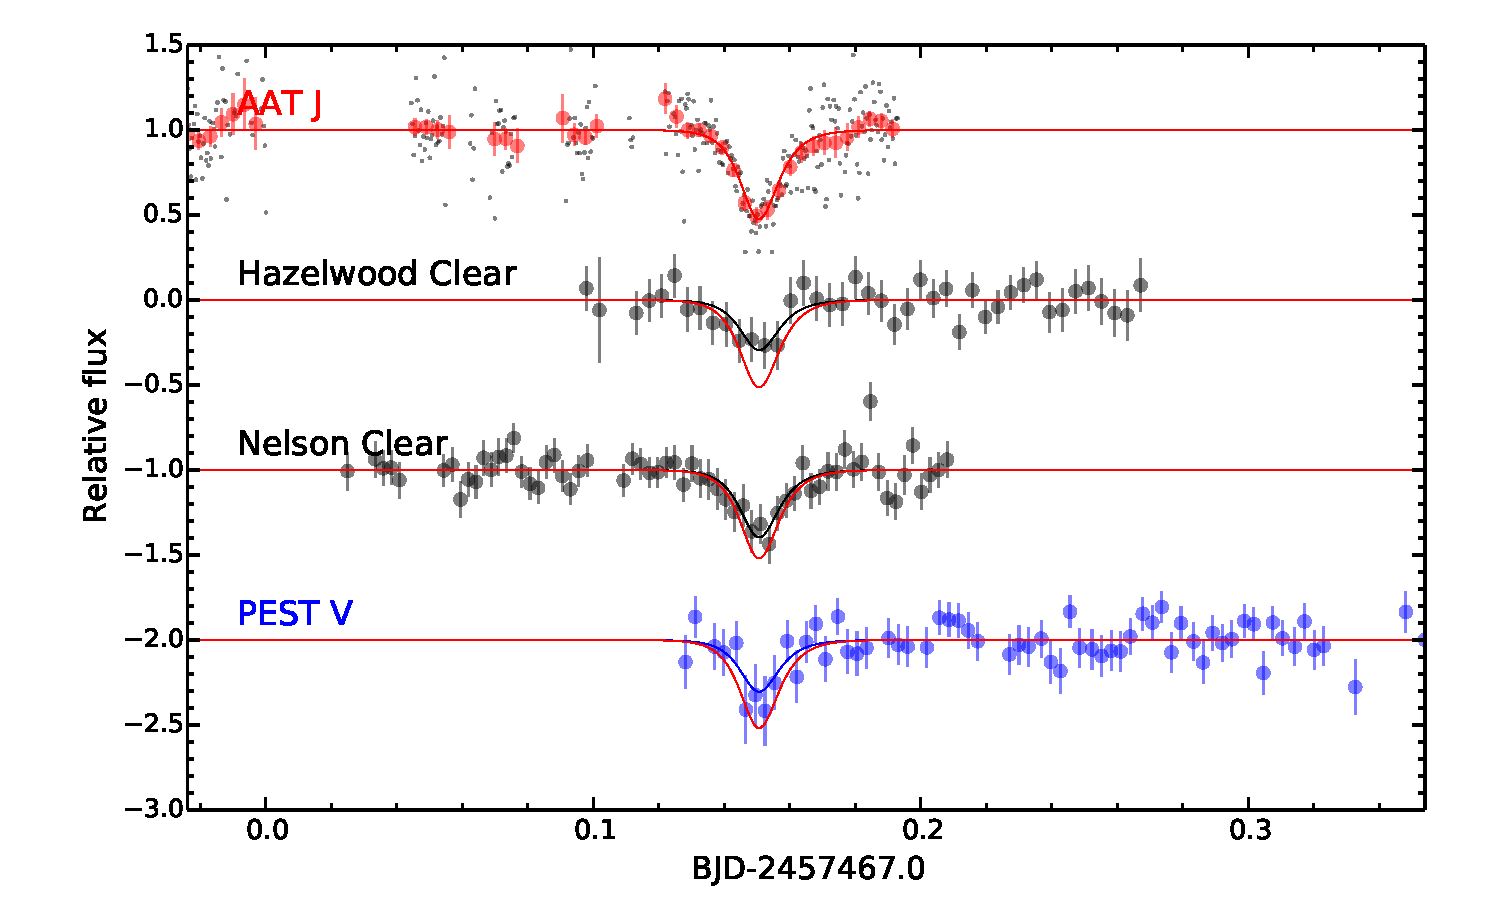
\includegraphics[width=18cm]{plots/20160319.eps}
    \caption{The light curves of WD1145+017 from 2016-03-19, simultaneous observed by the AAT in the infrared $J$ band, and by a series of small telescopes in the optical. The individual AAT observations are plotted in grey, and the 5 min binned light curve in red. The error bars in the bins represent the mean uncertainty of the points within the bin, scaled by the square root of the number of points per bin. The light curves of the optical facilities are shown at their native cadence. The shaded areas represent the $1\sigma$ region in the model fit. The solid lines show the best fit hyperbolic secant models. The optical light curves have their respective model fit regions, and the AAT model fit region (plotted in red) over plotted for comparison.}
    \label{fig:lc_20160319}
\end{figure*}

\begin{figure*}
    \centering
    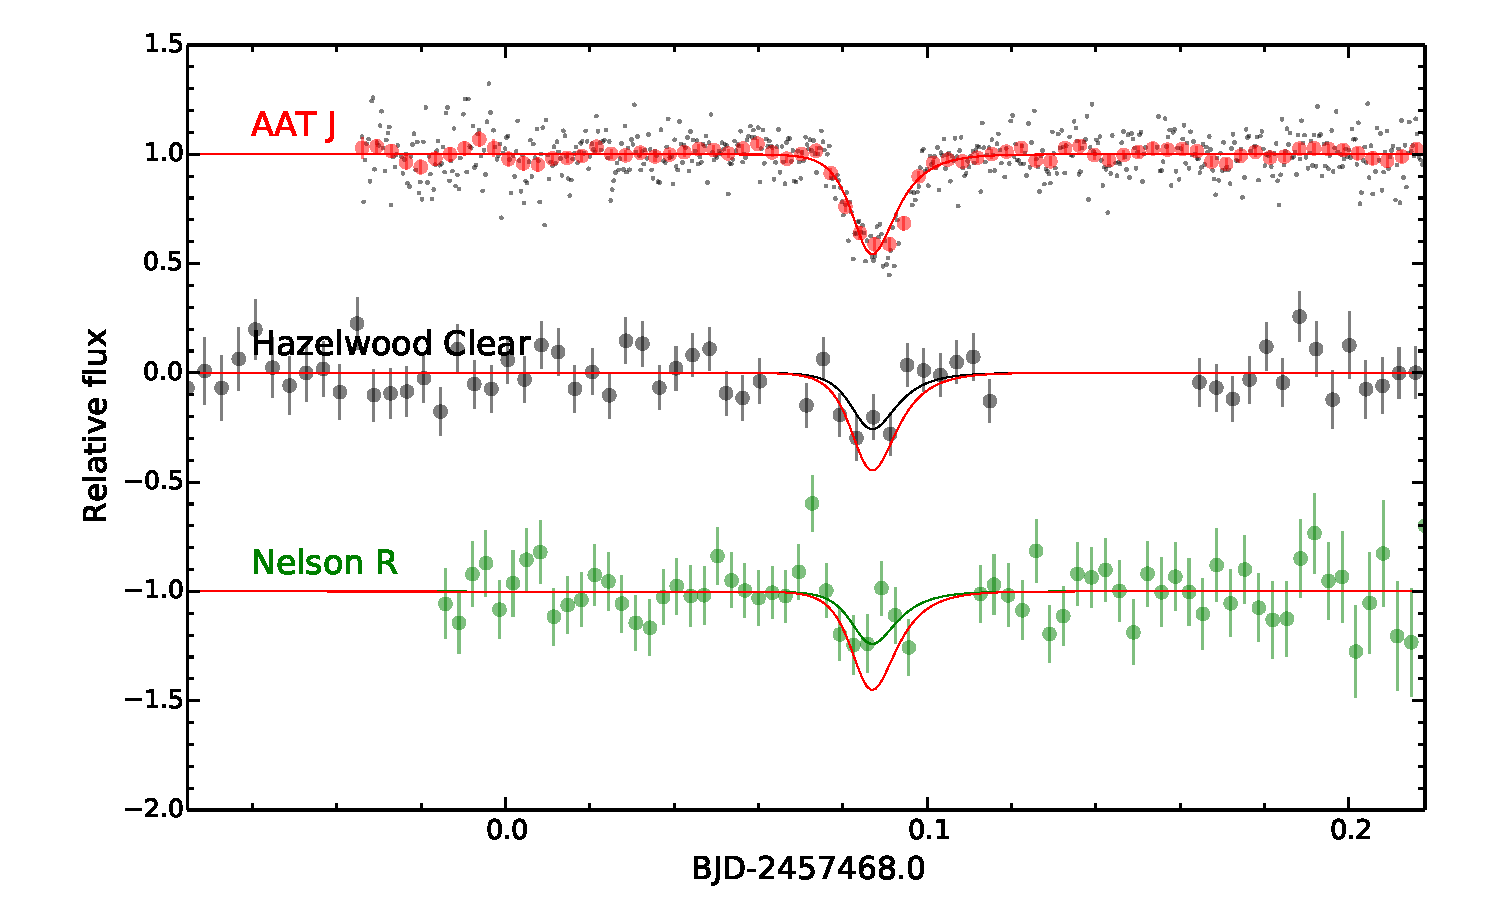
\includegraphics[width=18cm]{plots/20160320.eps}
    \caption{The light curves of WD1145+017 from 2016-03-20. See Figure~\ref{fig:lc_20160319} for description. }
    \label{fig:lc_20160320}
\end{figure*}

We measured no difference in the depth of the transit at difference photometric bands. Following \citet{2015arXiv151006434C}, the depth $D$, the minimum of the transit light curve, is given by 
\begin{equation}
D = C \frac{\zeta^{\zeta/(1+\zeta)} }{1+\zeta}\,,
\end{equation}
where $\zeta = \tau_2/\tau_1$. Figure~\ref{fig:depth_hist} shows the depth distribution of the transit at each band for each of the nights. In addition, the transit depth and shape shape were unchanged between the two nights, with $\tau_1 = 0.005\pm0.001$, $\tau_2 = 0.005\pm0.001$ on 2016-03-19 and $\tau_1 = 0.004\pm0.001$, $\tau_2 = 0.006\pm0.001$ on 2016-03-20. Interestingly, no significant asymmetry was measured for the transits [TDB: cite previous observations reporting asymmetry].

Given the lack of measurable change in the transit depth and and shape, we fit the data from both nights together, with all transits sharing the characteristic timescale parameters $\tau_1$ and $\tau_2$, and each band with independent depth parameter $C$. The reference transit time $\tau_0$ and transit period $P$ are also fitted for. The resulting transit depth distributions are plotted in Figure~\ref{fig:depth_hist}. We find no significant wavelength dependence of the transit depth when the datasets from the two nights are combined. The full set of derived parameter values are given in Table~\ref{tab:simultaneous_params}.

\begin{figure}
    \centering
    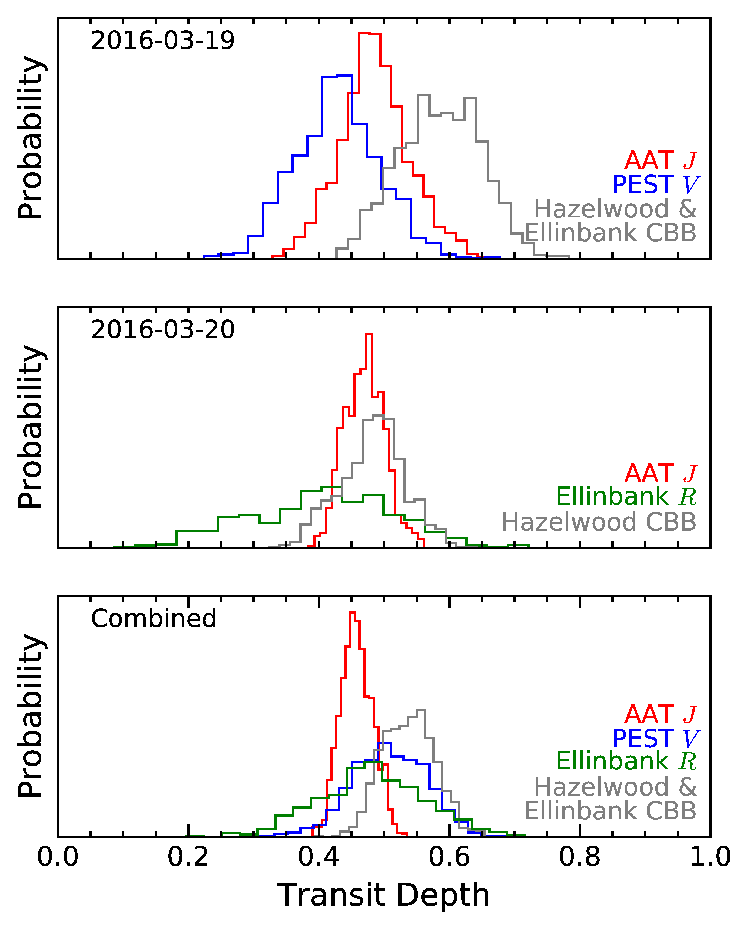
\includegraphics[width=7cm]{plots/depth_hist.eps}
    \caption{The transit depth $D$ distribution for the transits simultaneously observed at various photometric bands on 2016-03-19 (Top) and 2016-03-20 (Middle). The transits from each night were fit simultaneously, sharing the parameters governing the transit shape, but with different depths for each band. The transit depths agree with between each photometric band, and between the two nights, at the $1\sigma$ level. The bottom panel shows the depth distribution derive from fitting the data from both nights simultaneously, with all transit shape parameters shared, and per-band transit depth independent. Again, the transit depths from each photometric band agree to within $1\sigma$.}
    \label{fig:depth_hist}
\end{figure}

\begin{table*}
\centering
\caption{\label{tab:simultaneous_params}Transit parameters from multi-band simultaneous observations}
\begin{tabular}{lrrr}
\hline\hline
Parameter & 2016-03-19 & 2016-03-20 & Combined\\
\hline
\textbf{Fitted parameters} & & & \\
$\tau_0$ (BJD-TDB) & $2457467.150_{-0.001}^{+0.001}$ & $2457468.086_{-0.002}^{+0.002}$ & $2457467.1495_{-0.0009}^{+0.0010}$\\
Period (days) & ... & ... & $0.1874_{-0.0001}^{+0.0001}$ \\ 
$\tau_1$ (days) & $0.0045_{-0.0009}^{+0.0011}$ & $0.0039_{-0.0006}^{+0.0007}$ & $0.0037_{-0.0004}^{+0.0004}$ \\
$\tau_2$ (days) & $0.0055_{-0.0007}^{+0.0009}$ & $0.006_{-0.001}^{+0.001}$ & $0.0056_{-0.0006}^{+0.0007}$ \\
$C_J$ & $0.95_{-0.09}^{+0.10}$ & $0.91_{-0.07}^{0.05}$ & $0.88_{-0.04}^{+0.06}$ \\
$C_V$ & $0.9_{-0.1}^{+0.1}$ & ... & $1.0_{-0.1}^{+0.1}$\\
$C_R$ & ... & $0.8_{-0.2}^{+0.2}$ & $0.9_{-0.1}^{+0.1}$ \\
$C_\mathrm{CBB}$ & $1.2_{-0.1}^{+0.1}$ & $0.9_{-0.1}^{+0.1}$ & $1.04_{-0.09}^{+0.08}$ \\
\textbf{Derived depths} && \\
$D_J$ & $0.48_{-0.04}^{+0.05}$ & $0.47_{-0.03}^{0.03}$ & $0.46_{-0.02}^{+0.03}$\\
$D_V$ & $0.43_{-0.06}^{+0.06}$ & ... & $0.51_{-0.05}^{+0.05}$\\
$D_R$ & ... & $0.41_{-0.12}^{+0.09}$ & $0.48_{-0.08}^{+0.08}$\\
$D_\mathrm{CBB}$ & $0.59_{-0.06}^{+0.06}$ & $0.49_{-0.05}^{+0.04}$ & $0.54_{-0.04}^{+0.04}$ \\
\hline
\end{tabular}
\end{table*}

\subsection{Light curves from independent observations}

In addition to the simultaneous set of multi-band observations, we also obtained five nights of AAT $J$ band light curves in February 2016, and two nights of $g'$ band light curves in March 2016 with the LCOGT 1\,m network. 

Figure~\ref{fig:lc_201602} shows the light curves from the February AAT $J$ band observations. Two full transit events were observed on 2016-02-16 and 2016-02-21. The light curves were fit with the same procedure as per Section~\ref{sec:simultaneous_lc}, with the transit shape and depth assumed to be constant over the five nights. The transits were significantly shallower than those observed in March 2016, with depths of $D=0.17_{-0.03}^{+0.03}$ and significantly asymmetric ingress and egress timescales of $\tau_1 = 0.006_{-0.001}^{+0.001}$ and $\tau_2 = 0.0003_{-0.0003}^{+0.0003}$. In fact, the same hyderbolic secant model cannot fully model the ingress for the 2016-02-16 and 2016-02-21 transits. Fitting the two transit separately, we find the depth and shape to evolve over the 5 nights. The transit on 2016-02-16 has a depth of $D = 0.12_{-0.05}^{+0.14}$, $\tau_1 = 0.003_{-0.002}^{+0.004}$ and $\tau_2 = 0.001_{-0.001}^{+0.002}$, while the transit on 2016-02-21 was deeper and longer, with $D = 0.19_{-0.03}^{+0.03}$, $\tau_1 = 0.009_{-0.002}^{+0.002}$ and $\tau_2 = 0.0009_{-0.0004}^{+0.0006}$. The period derived from the transits $(P=0.18716_{-0.00003}^{+0.00003})$ is not significantly different from that in Table~\ref{tab:simultaneous_params} found in the March observations, but the transit centroid time in February is earlier than that in March by 0.029 days. 

\begin{figure*}
    \centering
    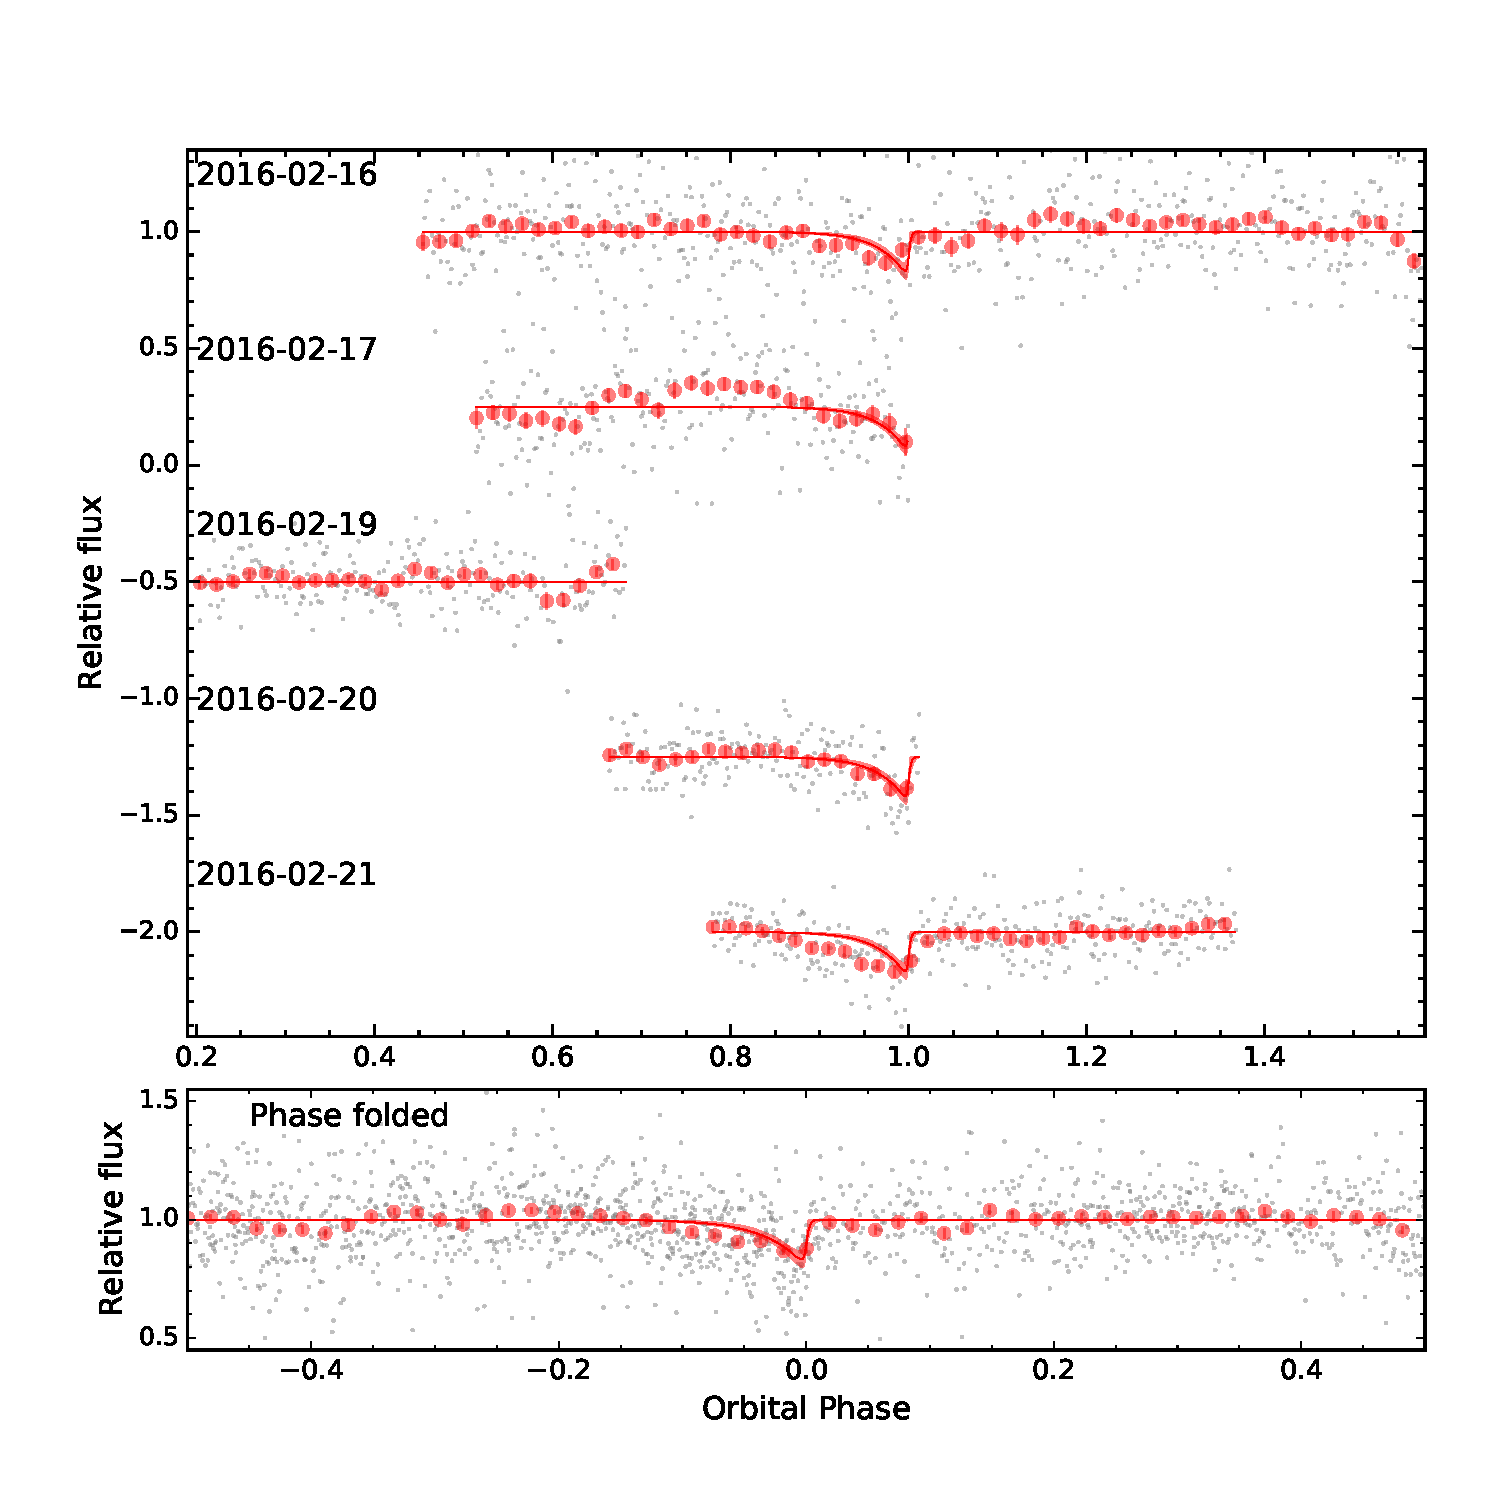
\includegraphics[width=18cm]{plots/AAT_feb.eps}
    \caption{WD1145+017 was monitored over five nights in February 2016 by the AAT in J band. Two full transit events were captured during this period. The individual AAT observations are plotted in grey, and the 5 min binned light curve in red.}
    \label{fig:lc_201602}
\end{figure*}

Observations were performed with the LCOGT 1\,m network on 2016-03-25 and 2016-03-28, $\sim 5$ nights after the AAT observations (Figure~\ref{fig:lcogt}). The system evolved significantly over the five days, with LCOGT light curves showing the two distinct transit event. We fit the light curves with a doublet transit, allowing for a shared $\tau_0$ and period. The primary component transits with a depth of $D = 0.45_{-0.02}^{+0.01}$, and exhibits some asymmetry with $\tau_1 = 0.002_{-0.0008}^{+0.0006}$ and $\tau_2 = 0.0052_{-0.0003}^{+0.0005}$. The secondary component has a shallower transit of $D = 0.21_{-0.01}^{+0.01}$, and exhibits some asymmetry with $\tau_1 = 0.0016_{-0.0003}^{+0.0003}$ and $\tau_2 = 0.006_{-0.002}^{+0.002}$. In both cases, the egress is longer than ingress, suggesting a trailing tail-like feature. The two transits are offset by $0.016_{-0.001}^{+0.001}$ days. The period derived from the dataset is $0.18725_{-0.00002}^{+0.00002}$ days, largely consistent with the period of the system at 2016-03-19/20. However, the transit centre of the primary event is delayed by 0.0048 days.  [TDB fit each separately]

\begin{figure*}
    \centering
    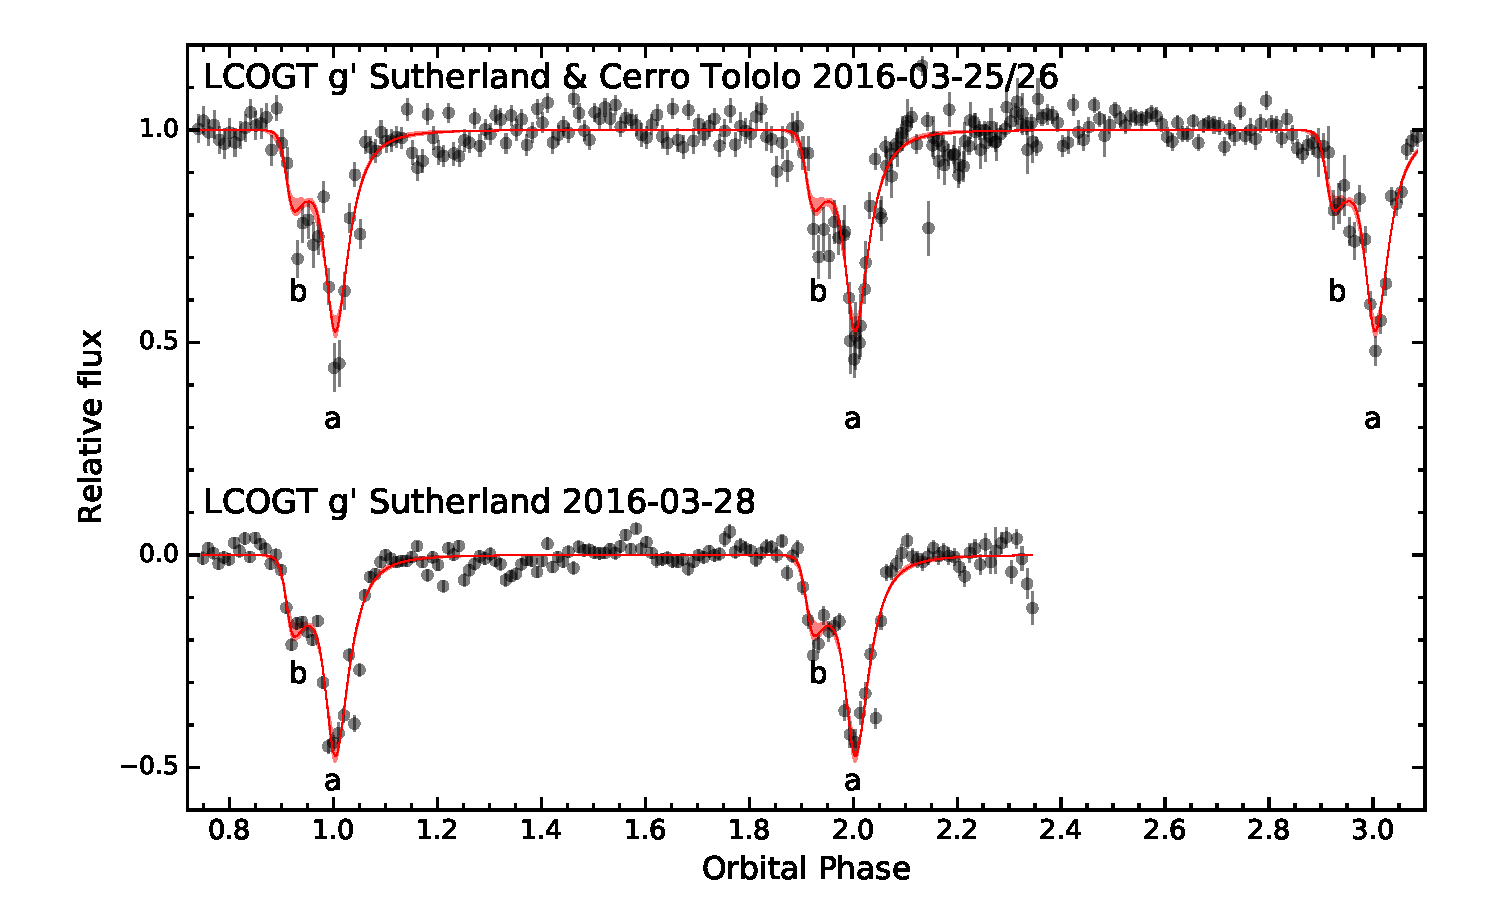
\includegraphics[width=18cm]{plots/lcogt.eps}
    \caption{$g'$ band light curves of WD1145+017 on 2016-03-25 and 2016-03-28, 5 days after the set of simultaneous observations. Four main transit events were observed over the two nights, each transit event involves a large 50\% event, and an adjacent 20\% event. The light curves were fit with a doublet transit model, allowing for $\tau_0$, period to be shared.}
    \label{fig:lcogt}
\end{figure*}

\section{Discussion}
\label{sec:discussion}

\subsection{Wavelength dependence}

Simultaneous observations for two transits of WD1145+017 were observed in the clear $CBB$, $V$, $R$, and $J$ bands on 2016-03-19 and 2016-03-20. The transit depths, derived from the combined set of light curves, are plotted in Figure~\ref{fig:band_depth}. We find no significant difference in the depth of the transits at different wavelengths. 

We calculate extinction cross sections for a power law distribution of spherical particles \citep[as defined by ][]{1974SSRv...16..527H} with effective radii from 0.05 to 20.0\,$\mu$m, and effective variance 0.1. The optical properties are those of "astronomical silicate" \citep{1984ApJ...285...89D,1993ApJ...402..441L}. The extinction was calculated using the Lorenz-Mie scattering code of \citet{2002sael.book.....M}. The lack of wavelength -- transit depth dependence is consistent with particle size of $\gtsim 1\,\mu$m, consistent with previous studies [cite]. Figure~\ref{fig:band_depth} shows a selection of the models, from 0.5 to 5.0\,$\mu$m, normalised to the $J$ band transit depth.

\begin{figure}
    \centering
    \includegraphics[width=7cm]{plots/band_depth.eps}
    \caption{The transit depths of WD1145+017 at the $CBB$, $V$, $R$, and $J$ photometric bands, as measured from simultaneous observations on 2016-03-19 and 2016-03-20. We find no wavelength dependence for the transit depth. Extinction curves for particles 0.5 to 5.0\,$\mu$m are plotted for comparison. The particule sizes can be constrained to be $\gtsim 1\,\mu$m.}
    \label{fig:band_depth}
\end{figure}

[From Jonty: From the WD luminosity (121 L_sol), the minimum (blow-out) grain size should be ~ 11.8 um, so we’d be well into the flat regime for the dust grains on that basis. Putting this size constraint into a simple power law sixe distribution astrosilicate dust model gives the attached SED, assuming astrosilicate dust varying in size from 11.8um to 1mm with a size distribution exponent of 3.5 (dn = a^-x da) in a narrow dust belt (dr/r = 0.1) at a semi-major axis equivalent to a 4.5 hr period (5x10^-3 au). ]

\subsection{Transit timing variation}





\acknowledgments
acknowledgments

Facilities: \facility{AAT}

\bibliographystyle{mnras}
\bibliography{mybibfile}

\end{document}
